\documentclass[a4paper,11pt]{article} 
\usepackage[french]{babel}
\usepackage[T1]{fontenc} 
\usepackage[utf8]{inputenc} 
\usepackage{graphicx}
\usepackage{color}
\usepackage{hyperref}
\usepackage{array}
\begin {document}
\begin {figure}
\includegraphics[width=0.3\textwidth]{logolemansU.png}
\hspace{150pt} 
\includegraphics[width=0.3\textwidth] {logo_ic2.png}
\end {figure}
\title {\textbf {\color {blue} Le Mans Université}\color{black}
\\  Licence Informatique  \textit {2ème année}
 \\Module Conduite de Projet
 \\ \textbf {Battle Ground }}
\author{
{\href{mailto: Lazare.Maclouf.etu@univ-lemans.fr} {Lazare Maclouf}} \and
{\href{mailto: Geoffrey.Pose.etu@univ-lemans.fr} {Geoffrey Pose}} \and
{\href{mailto: Valentin.Charretier.etu@univ-lemans.fr} {Valentin Charretier}} \and 
{\href{mailto: Mathieu.Brière.etu@univ-lemans.fr} {Mathieu Brière}}
}
\date{\today} 
\maketitle 
\newpage
\tableofcontents
\newpage
\section {Introduction}
\\Dans le cadre du module "conduite de projet" de notre deuxième année de licence Informatique. Nous avons décidé de développer un jeu différent des sujets proposés (mots-mêlés, othello...), nous avons donc décidé de créer notre propre jeu, en le nommant "Battle Ground". En nous inspirant de jeux déjà existant, et en développant certains modes de jeu pré-existant, nous avons décidé de prendre ces idées et d'appliquer nos propres règles.
\\ En l'occurrence, ici, deux jeux nous ont servis de base de travail : "Age of war" et "Plant vs zombies 2". Ces deux jeux sur mobiles partagent deux systèmes en commun : le joueur doit défendre sa base face aux incessantes attaques de l'ennemi, ainsi que la gestion économique des ressources pour défendre plus facilement la base ou avoir de meilleures entités.
Pour le jeu "Plant vs zombies 2", le joueur doit défendre sa base en y installant des plantes qui sont utilisées comme tourelle de défense. Le but est de survivre le plus longtemps possible face à des vagues constantes d'ennemis prédéfinies par l'ordinateur.
Quant au jeu "Age of war", il fonctionne différemment ; le mode de jeu est un 1 contre 1. Le but est de détruire la base ennemie, tout en gardant sa propre base en vie en la défendant du mieux possible. Il y a deux types d'entité dans le jeu, les tourelles, qui sont destinées à défendre la base en éliminant la moindre unité rentrant dans la portée des tirs. Et des unités qui ont pour objectif la destruction de la base ennemie, tout en éliminant les unités hostiles sur leur chemin. De plus, le joueur ennemi est une IA possédant les mêmes caractéristique que le joueur humain. Mais a contrario, l'IA reçoit certains avantages selon la difficulté (plus d'argent, plus d'expériences, et tout autres bonus comme le nombre de points de vie).
Le jeu que nous avons créé reprend les concepts des deux jeux, c'est-à-dire: le système de vague ainsi que le mode 1 contre 1.
Le joueur a donc une base à défendre avec la possibilité de créer une tourelle et des unités. Cependant, l'ordinateur en face de lui ne joue que des vagues comme dans prédéfinis.
Notre groupe est composé de quatre personnes Mathieu Brière, Lazare Maclouf, Valentin Charretier et Geoffrey Posé.\\
Nous verrons dans ce rapport quel ont été les outils utilisés dans la réalisation du jeu, ainsi que les différentes étapes de création du jeu "Battle Ground".\\
En premier lieu, nous aborderons la conception du jeu, suivi de la présentation des différents outils utilisés ainsi que leur rôle dans la gestion du projet. Par la suite, nous verrons toute la phase de développement du projet ; nous terminerons par les résultats obtenus. Et pour conclure, nous dresserons un bilan de ce qui a fonctionné dans le développement du projet, et de ce qui n'a pas, ou peu été utilisé dans le projet pour de multiples raisons.\\
\section {Conception du jeu}
\subsection {Règles du jeu}

Plusieurs modes de jeu ont été choisis :\\

-Le mode "survivant" : comme son nom l'indique, le joueur devra se défendre face à une suite de vagues constante d'unité ennemie. Le joueur perd une fois que sa base n'a plus de point de vie. À l'inverse, le joueur gagne s'il réussit à tenir face aux vagues ennemies et s'il lui reste des points de vie.\\

-Le mode "classique" : initialement, il devait s'agir d'un mode où le joueur joue contre l'ordinateur. Cependant, par manque de temps à la création d'une IA viable, nous avons pris la décision d'en faire un mode de 1 contre 1 sur le même ordinateur où les deux joueurs jouent avec la même souris.\\

\subsection {Options du joueur}
\begin{figure}[ht!]
\centering
\includegraphics [width=1\textwidth]{image9.jpg} 
\caption {\label{image1} options du joueur en pleine partie}
\end{figure}
 \smallbreak
Durant une partie, le joueur a plusieurs options :\\

-Créer des unités : le joueur a la possibilité de créer différentes unités aux caractéristiques uniques, qui vont défendre la base et attaquer les entités ennemies sur leur chemin. En contrepartie, le joueur dépense une certaine somme d'argent pour pouvoir les créer.\\

-Créer une tourelle : une fois installée sur la base, elle se met à tirer sur les entités ennemies rentrant dans leur porté d'attaque. Lorsque le niveau est terminé (en mode survivant), la tourelle, si elle a été installée, est supprimée.\\

-Mise en pause : le joueur peut mettre en pause la partie et la reprendre quand il le souhaite. Il lui suffit d'appuyer sur le bouton pause en jaune, au milieu en haut de l'écran.\\

-Quitter la partie : à tout moment, le joueur peut quitter la partie, ce qui n'est pas une fonctionnalité en soit. Cependant, lorsqu'il souhaite quitter la partie, un message d'alerte s'affiche à l'écran ; et le joueur est informé que la partie ne sera pas sauvegardée.\\

\subsection {Jouabilité et fonctionnalités du jeu}
\\
En premier lieu, lors du lancement du jeu, un menu s'affiche à l'écran avec comme options "jouer", "paramètres", "quitter".
\begin{figure}[ht!]
\centering
\includegraphics [width=1\textwidth]{image1.jpg} 
\caption {\label{image2} menu principal}
\end{figure}
 \smallbreak
Lorsque le joueur clique sur quitter, le jeu se ferme instantanément. Lorsqu'il clique sur jouer, un autre menu s'affiche alors ; avec les différentes options suivantes : "survie", "classique", "retour". "Survie" lance une partie en mode survivant, retour fait revenir le joueur au menu précédent (fonctionnalité entourée en rouge sur la photo du jeu). Et "classique" renvoie vers un autre menu demandant de choisir la difficulté avant de lancer la partie.
\begin{figure}[ht!]
\centering
\includegraphics [width=1\textwidth]{image2.jpg} 
\caption {\label{image3} sous menu jouer}
\end{figure}
 \smallbreak
Quand partie est lancée, une palette de boutons en haut de l'écran correspondant aux unités disponible d'utilisation, à la tourelle que l'on peut installer, à la fonctionnalité retour au menu et enfin à la fonctionnalité mettre en pause (entourée en rouge sur la photo ci-dessous).
\begin{figure}[ht!]
\centering
\includegraphics [width=1\textwidth]{image3.jpg} 
\caption {\label{image4} photo du jeu en mode survivant}
\end{figure}
 \smallbreak
En haut à gauche de l'écran, il y a également la somme totale d'argent du joueur pouvant être utilisé durant la partie. Ce dernier commence la partie avec 1000 pièces et en collecte 250 par unités tuées. Grâce à ces pièces, il peut créer des unités en payant le prix affiché en dessous de chaque case. Nous nous attendons à avoir une fluidité plus ou moins correcte sur la vitesse de la partie. La marge d'erreur dépendant du système d'exploitation et surtout du processeur (globalement un peu plus fluide sur Windows que sur Linux). 

\section {Outils Utilisés}
Différents outils ont été utilisés lors de la création du jeu pour facilité certaines étapes du processus.
\subsection{GCC}
Il s'agit du compilateur utilisé pour générer un exécutable à partir du code source. De nombreuses options sont disponibles notamment pour le débuggage ou pour préciser une librairie spécifique à inclure pour la compilation. Il est compatible avec Windows, Mac-OS et Linux.
\subsection{GDB}
GDB est un débugguer pour le langage c, il a permis de voir l'origine de nombreuses erreur de segmentations (en grande partie liées aux listes chaînées).\\
\subsection{Doxygen}
Il s'agit de l'outil de documentation de code qui a été utilisé pour générer des schémas et graphes pour mieux comprendre les dépendances et interaction des fonctions grâce à un balisage minutieux du code source au préalable. \\
\subsection{Discord}
Cela a été notre moyen de communication principal durant le projet. En effet, nous avons créé une conversation de groupe ce qui a été très pratique pour échanger sur diverses choses concernant le projet. Discord étant une des applications les simples d'utilisation et efficace pour communiquer rapidement avec plusieurs personnes.\\
\subsection{GitHub}
GitHub a été l'hébergeur de notre projet, c'est une plateforme gratuite regroupant beaucoup d'outils et de programmes codés sous divers langages. C'est dessus que l'ensemble des fichiers du projet sont stockés (du code source jusqu'à la documentation sans oublier les librairies, le makefile et les fichiers de ressources du jeu).\\
\subsection{Atom et Visual studio code}
Ces deux outils sont plus ou moins similaires et servent tout deux d'éditeur de texte spécifique à la programmation. Très pratique et gratuit, c'est dessus que nous avons codé le jeu. Visual studio code a la particularité d'avoir un environnement plus complet que son rival, tout deux possède des outils facilitant la vie du développeur et permet des raccourcis (reconnaître une fonction et donner la doc en rapport avec réorganiser et indenter le code pour qu'il soit lisible, etc.).\\
\subsection{Valgrind}
Valgrind a permis de vérifier tout au long du développement du projet, que le jeu n'avait pas ou peu de fuites de mémoires (finir avec 0 fuite de mémoires est un véritable challenge). Pour ainsi nous assurer que le jeu était correctement optimisé et n'allouait pas de la mémoire inutilement, et bien sûr sans oublier de libérer cette dernière, pour pouvoir la ré-alouer plus tard sans erreur de données dans le futur.\\
\subsection{Paint.net}
Il s'agit d'une version améliorée et plus poussée de paint. L'utilisation de ce logiciel a eu pour but réalisé les décors, les entités ainsi que tout autre élément à afficher. En effet, les possibilités sont beaucoup plus grandes dans la réalisation d'image et de leur modification ; comme par exemple : nous pouvons y ajouter du texte, faire des superpositions, découper des partie d'image, modifier les couleurs ou encore de dessiner avec diverses formes géométriques possibles. Enfin, pour ce qui est du format, nous avons eu la possibilité d'enregistrer les images sous divers formats (bmp, png, jepg, gif), pour réduire la taille des documents, ainsi que d'avoir une meilleure qualité sur les différentes images. Cela a très été utile pour toute la partie graphique du jeu.\\
\subsection{Gimp}
Gimp est un outil plus ou moins similaire au précédent avec quelques particularités différentes. Ces deux logiciels ont été utiles, car dans certains cas spécifiques, nous avons pu réussir à modifier, créer les images de la bonne façon en variant les logiciels. L'utilisation de deux logiciels différents pour la création des graphismes a été un atout puissant dans la création du jeu.\\
\subsection{Cyotek spriter}
C'est un outil servant à créer un unique sprite à partir de plusieurs images. En effet, avec des images séparées sur lesquelles on a une position unique à chaque image, cyotek spriter permet d'assembler plusieurs images indépendantes sur un seul et même sprite complet.\\ 

\section{Gestion du projet}
\subsection{Organisation des tâches}

Geoffrey Posé s'est occupé de générer le Doxygen final à l'aide de l'outil Doxygen ainsi qu'à organiser et créer une arborescence lisible, claire et structurée du code. Il s'est occupé de corriger certains warnings dans le code au fur et à mesure de l'avancement du projet et a créé la page internet sur laquelle nous avons pu faire notre diagramme de Gantt et la \href{https://mat7813.GitHub.io/Battle-ground/doc/html/index.html}{Documentation}. Il nous a aidé pour configurer entièrement le GitHub et à bien définir les environnements de travail (création de branches). Il a pu nous aider au tout début à configurer git. Il a également produit un mode de jeu en un contre un  sur le même ordinateur.\\ 

Mathieu Brière a créé le git sur lequel le jeu a été déposé avec tous les fichiers qu'il comprend. Il s'est occupé de trouver et de modifier les sprites du jeu (par exemple les tourelles, les entités et autres affichages comme les pièces, inventaire, icon, ...) . Il a modifié les boutons des différents menus ainsi que de multiples modification de plusieurs fichiers .c. Il a aussi codé le fichier audio.c grâce auquel la musique du jeu, à l'aide de la librairie SDL mixer. Ainsi que d'avoir travaillé sur la réalisation du mode "multi" pour que deux joueurs puissent jouer à distance en réseau. Ainsi que de la réécriture du rapport.\\

Lazare Maclouf a codé les fichiers c excepté le fichier audio.c et classique.c. , incluant les primitives grâces auxquelles le jeu fonctionne, l'interface graphique, la gestion des menus, les animations des entités, le mode survivant, les structures (joueur, entite, wave, msg, defense etc..), la gestion de l'environnement, du comportement des entités, de leur cohérence de déplacement, etc... Il s'est occupé de rédiger le rapport final en latek. Il a trouvé, modifié et créé les images des décors, des entités bandit, mumma et voisin ainsi que pour l'argent, les cadres, les menus et les boutons (avec l'aide de Mathieu Brière). Il a également créé les images contenant des polices d'écritures 3D (les images comme survivant, vous n'avez pas assez d'argent, etc..). \\

Valentin Charretier a travaillé sur les socket, pour tenter de créer un mode multijoueur. Ce qui aurait ainsi offert la possibilité de jouer en un contre un avec deux ordinateurs distincts.\\

\subsection{Ajouts de tâches au fur et à mesure}
Nous avons remarqué que le Gantt prévisionnel n'était pas parfait. En effet, de nombreuses tâches pour développer le jeu étaient manquantes. C'est pourquoi sur le Gantt effectif, nous avons rajouté les différentes tâches qui manquaient (tests, étapes supplémentaires pour coder le jeu...) au fur et à mesure de l'avancée du projet. On ne se rendait compte du besoin de certaines tâches qu'une fois en train de développer concrètement le jeu et qu'avant cela, il était difficile de répertorier et de lister tout ce qu'il fallait faire pour créer le jeu.\\

\section{Développement}
Le jeu a été codé en utilisant les différentes librairies composées de : SDL2, SDL2 image ainsi que de SDL mixer pour l'audio.

\subsection{Structures utilisées}
Plusieurs structures ont été initialisées pour le bon fonctionnement du jeu.\\ 

\begin{figure}[ht!]
    \centering
    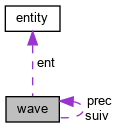
\includegraphics [width=0.2\textwidth]{struct wave.png} 
    \caption {\label{image5} liste chaînée}
    \end{figure}
     \smallbreak

Les structures entite, wave et joueur par exemple, sont essentielles lors du déroulement d'une partie. En effet, une wave~\ref{image5} est une liste chaînée d'entité comportant chacune de nombreux paramètres. Parmi eux, nous pouvons y retrouver la valeur de l'abscisse et l'ordonnée de la barre, ainsi que de l'entité, ses points de vie, son nombre de dégâts, une chaîne de caractère correspondant à l'entité pour l'animer, etc. Ces structures sont gérées grâces à des primitives, contenues dans le fichier vague.h. Toutes les fonctions de création d'une structure entité ou vague, du déplacement dans la liste chaînée, ainsi que de leur suppression, se trouve dans ce fichier. La structure joueur par exemple, contient les informations relatives au joueur comme son argent, ses points de vie ou toute autre information liée au joueur. Certaines structures peuvent paraître très longues (avec beaucoup de paramètres). Toutes ses décisions vont être justifiées dans les points suivants.

\begin{figure}[ht!]
    \centering
    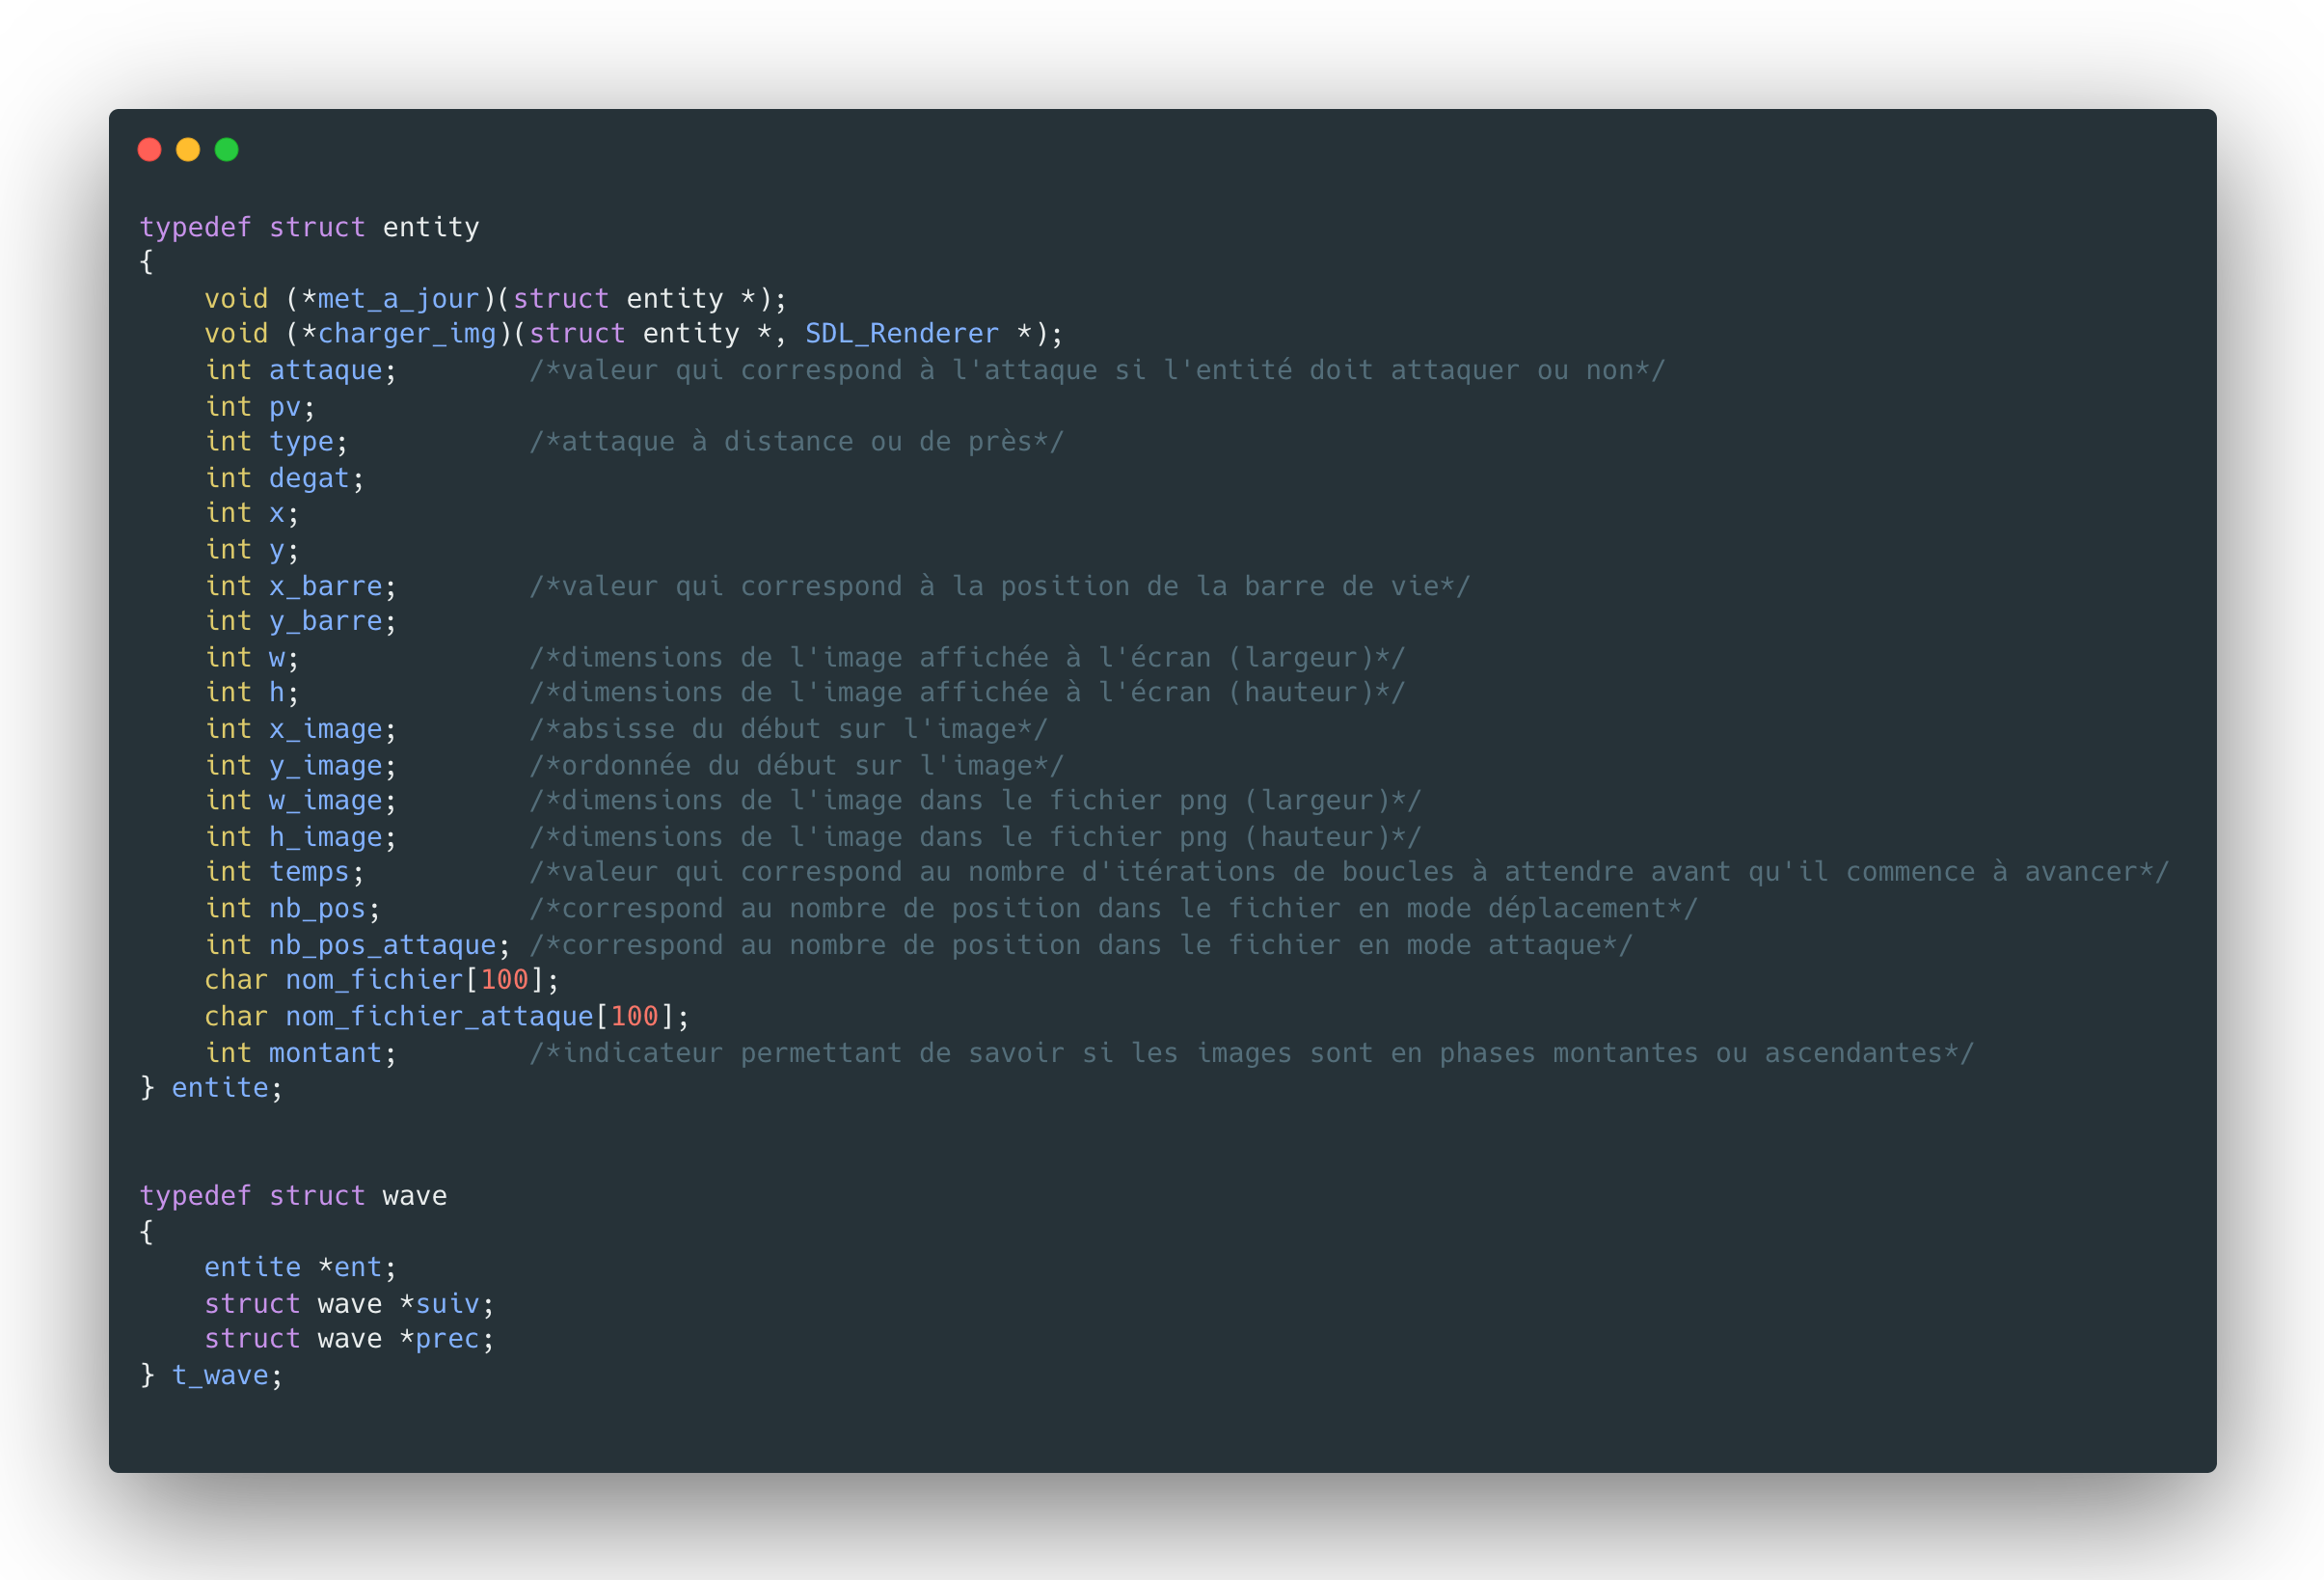
\includegraphics [width=1\textwidth]{wave.png} 
    \caption {\label{image5} structures vague et entitée}
    \end{figure}
     \smallbreak

\subsection{Interface graphique avec SDL et SDL image}
La bibliothèque SDL ne peut, par défaut ; Que charger sur le rendu et afficher sur la fenêtre des images au format bmp.\\ Pour remédier à cela et afficher des images avec tout type d'extension, il a fallu utiliser la librairie SDL image. Toutes les fonctions relatives à l'interface graphique (affichage des menus, des images, etc.) se trouvent dans le fichier interface.c, elles sont utilisées dans le reste du code lors de la gestion d'une partie par exemple.\\ Plutôt que de charger un tableau de textures en variable globale dans tout le jeu. Des fonctions indépendantes se chargent de toutes les étapes pour afficher une image à l'écran. De la création de la texture, jusqu'à la copie sur le rendu.

\subsection{Animations des unités et des tirs}
\subsubsection{Technique d'animation des entités}
Deux techniques d'animation ont été utilisées pour animer les entités.\\ La première consiste à charger successivement plusieurs images différentes sur lesquelles on a une position différente à chaque fois.\\ La deuxième consiste à charger une partie d'une image comportant toutes les positions successives d'une entité ou d'un objet (sprite) et à se déplacer dans le fichier pour charger les différentes positions de l'entité.\\ Étant tombé sur des entités avec des images différentes, le plus simple a été d'incorporer les deux méthodes d'animations au jeu.

\subsubsection{Fonctionnement des animations globales}
La SDL fonctionne avec à un seul et unique rendu pour une fenêtre sur laquelle on affiche ce qu'on veut. Ainsi, si l'on souhaite afficher un décor avec une unité bougeant dessus, il suffit simplement de superposer le décor, l'unité et donc les charger dans le bon ordre. Pour la faire bouger, il faut à chaque fois tout supprimer et tout recharger. \\ Plusieurs problèmes ont été rencontrés :\\ -Un clignotement de certaines parties des images une fois affichées à l'écran (dû à une mauvaise gestion de l'ordre d'affichage)\\ -Une synchronisation dans un premier temps de l'animation des entités lorsqu'elles sont plusieurs à se déplacer en même temps sur l'écran.\\

Pour régler ces problèmes, les structures dont on a parlé plus haut, on été mises en place. \\ Concrètement avant d'afficher le rendu final à l'écran, dans la fonction gérant la partie (pour le mode survivant par exemple), on parcourt toute la liste chaînée d'entité, pour laquelle chaque position est enregistrée et mise à jour. Si une entité est créée après une autre, son animation ne sera pas la même que la précédente. Une fois parcouru toute les listes chaînées et charger les images successivement sur le rendu, puis en dernier, on charge les images relatives au bouton, à l'affichage en haut (cadre dans lequel il y a les unités, le bouton pause, retour, etc..). Cela permet ainsi une indépendance complète entre les entités.

\subsubsection{Animation des tirs}
Comme pour l'animation des entités, une structure tir a été définie pour pouvoir animer indépendamment le tir des autres éléments du décor avec le même procédé que pour les entités, à la différence qu'il n'y a qu'un seul tir à la fois.

\subsection{Gestion de l'environnement et des unités}

De nombreux éléments pour avoir un jeu cohérent et fonctionnel ont été à prendre en considération et à faire. La vitesse de déplacement des entités, des tirs, l'arrêt d'une entité lorsqu'elle est devant un obstacle ou une autre entité... Pour ce faire, il a fallu faire des fonctions vérifiant pour chaque entité (en parcourant à chaque fois la liste chaînée d'entité complètement) leur position relative aux autres entités ainsi que leur position absolue afin d'éviter qu'une entité ne continue à avancer et par conséquent sortir de l'écran ou passer à travers une autre entité. Toujours dans les structures, des indicateurs de type int ont été mis en place afin de pouvoir ordonner l'arrêt d'une entité ou son mouvement lors de l'utilisation des fonctions d'affichages. Il existe deux types d'entités au sein du jeu : les entités courtes et longues portées.

\begin{figure}[ht!]
\centering
\includegraphics [width=1\textwidth]{image4.jpg} 
\caption {\label{image7} niveau 2 partie survivant}
\end{figure}
 \smallbreak
Lors de la gestion des lignes d'entités, il faut prendre en considération la distance relative aux autres unités pour savoir si elle peut avancer ou si elle doit s'arrêter, mais aussi pour savoir quand déclencher les attaques. Pour pouvoir ainsi faire jouer ces deux types d'entité en harmonie, il a fallu que les fonctions de gestion de l'environnement prennent en compte le type pour chaque entité et ainsi agir en conséquence (toujours avec un paramètre spécifique relatif dans la structure). Ainsi, une bonne jouabilité et respectant ses propre lois physiques, un dynamisme des objets animés ainsi qu'une cohérence dans leur comportement (arrêt des entités face à un obstacle, reprise de déplacement lorsque la voie est libre, attaque lorsqu'une entité ou une base est à portée de main...).

\subsection{Structure des fichiers et des fonctions principales}
\begin{figure}[ht!]
\centering
\includegraphics [width=1\textwidth]{image5.jpg} 
\caption {\label{image8} schéma sur la hiérarchie des fichiers entre eux}
\end{figure}
 \smallbreak
Le code source du jeu est composé de 9 fichiers C ainsi que 9 fichiers H.

\subsection{Tests}
Lors de la création du jeu, de nombreuses fonctions pour manipuler les structures de données, on été faites. Comme ces structures sont manipulées avec des pointeurs, si les fonctions ne sont pas correctement réalisées, cela peut donner lieu à des erreurs de segmentation.
\begin{figure}[ht!]
\centering
\includegraphics [width=1\textwidth]{image6.jpg} 
\caption {\label{image9} dossier de test}
\end{figure}
 \smallbreak
C'est pourquoi des tests ont été faits pour l'utilisation de chacune de ces fonctions jusqu'à ce qu'elles fonctionnent parfaitement dans des fichiers à part, séparés du code source du jeu. D'autres tests pour la SDL ainsi que pour les fichiers audio ont également été faits.

\section{Bilan}
\subsection{Résultats}

Le jeu fonctionne globalement, correctement. Nous avons dans l'ensemble, fait différemment du diagramme de Gantt de départ.\\ En effet, nous avons fait face à plusieurs imprévus et aspects que nous n'avions pas pus anticiper. Pour ce qui est de l'affichage, la SDL ne pouvant que simplement charger à l'écran, en lui demandant simplement de charger et de superposer les images, il a fallu élaborer une méthode d'animation et d'affichage comme vu plus haut. Nous nous s'étions également trompés sur le temps que chaque tâche allait nous prendre. Les phases de test ont été beaucoup plus longues que prévues. Avant d'avoir des structures de données et des primitives qui manipulent ces structures fonctionnelles, il a fallu du temps et beaucoup de tests ainsi que de débuggage avec gdb. Ne plus avoir d'erreur de segmentation n'a pas été chose facile.
De plus, la coordination des éléments dans le jeu a été plus compliquée que prévue elle aussi. En effet, il a fallu voir et revoir les fonctions de chargement pour l'affichage des différents éléments, afin de les placer dans le bon ordre, au bon moment et au bon emplacement sur l'écran. Pour ce qui est des boutons durant une partie, réussir à bien détecter au bon moment le passage de la souris et au bon endroit, ont été une vrai difficulté, car les autres fonctions (celles qui gèrent le joueur, les entités et autres) sont appelées en permanence. Lorsque le programme se trouve dans une fonction, cela le bloque temporairement dans ce qu'il est en train de faire, ce qui peut empêcher l'exécution de choses en parallèles l'utilisation de threads pour y remédier peut être utile comme nous le verrons dans les améliorations.
Potentielles ci-dessous. Il a fallu donc calibrer et placer les instructions dans le bon ordre. Ces défauts ont ainsi pu être corrigés en partie avec une bonne structure du code. \\ L'équilibrage du jeu n'est pas optimal. Le jeu est en partie déséquilibré et on peut gagner à tous les coups avec la même stratégie. Le potentiel d'action de l'utilisateur est limité ce qui n'offre pas une très grande expérience de jeu.\\\\ 


\begin{figure}[ht!]
\centering
\includegraphics [width=1\textwidth]{image10.jpg} 
\caption {\label{image10} Gantt Prévisionnel partie 1}
\end{figure}
 \smallbreak

En comparant le Gantt prévisionnel et le Gantt effectif, on peut voir que de nombreuses tâches n'avaient pas été anticipées et le nombre d'heures prévues pour les effectuer étaient souvent mal jugées (sous-estimées ou sur-estimées). Comme on peut le voir sur les deux photos  représentant le Gantt effectif, de nombreuses tâches ont été réalisées à cent pour cent, ce qui est une bonne choses du point de vue de l'organisation. Cependant, on peut aussi voir des tâches inachevées, telles que l'interface graphique du mode classique pour ne citer que la partie visible. Ou encore, des tâches malheureusement non effectuées, soit par manque de temps, soit par remplacement d'une autre ou même que ces taches deviennent obsolète dans le projet.

\begin{figure}[ht!]
\centering
\includegraphics [width=1\textwidth]{image11.jpg} 
\caption {\label{image11} Gantt Prévisionnel partie 2}
\end{figure}
 \smallbreak
\begin{figure}[ht!]
\centering
\includegraphics [width=1\textwidth]{image7.jpg} 
\caption {\label{image12} Gantt effectif partie 1}
\end{figure}
 \smallbreak
\begin{figure}[ht!]
\centering
\includegraphics [width=1\textwidth]{image8.jpg} 
\caption {\label{image13} Gantt effectif partie 2}
\end{figure}
 \smallbreak



\subsection{Améliorations potentielles}


Comme nous avons pu le constater le jeu n'est pas fonctionnel à cent pour cent.\\ Plusieurs petits problèmes d'affichage sont encore présent, ainsi que des petits problèmes de fluidité par moment. Pour ce qui est de la jouabilité, elle peut être encore améliorée. C'est-à-dire que tout ce qui concerne l'équilibrage du jeu, incluant la difficulté, les possibilités du joueur, les événements imprévus (avalanches de météorites qui détruisent les unités) pourrait être grandement peaufiné. Cela donnerait une expérience beaucoup plus variée et riche à l'utilisateur. La plupart des jeux de stratégie dans "Age of war" ou "Plants vs zombies" présentent un panel d'options et de possibilités réduites pour se défendre et attaquer. Ce qui fait que l'utilisateur n'a aucune garantie de gagner, en utilisant juste une seule méthode particulière et doit rester attentif du début jusqu'à la fin de la partie. Concrètement, pour ce qui est de la défense, nous pourrions faire en sorte qu'à chaque niveau, il y ait beaucoup plus de types d'unités différentes et avec une fréquence variable. Le manque de diversité d'entités qui attaquent le joueur est notable au niveau de l'expérience utilisateur. De plus, il suffit de suivre une seule stratégie pour gagner. En effet, en plaçant la même unité au bon moment régulièrement et de continuer jusqu'à la victoire rend le jeu nettement plus désuet.\\
Nous pourrions faire également en sorte que le jeu soit beaucoup plus optimisé et opérationnel, en chargeant par exemple un tableau de textures directement au début du jeu plutôt que de recharger à chaque fois l'image que l'on souhaite afficher. De plus, nous pourrions scinder toutes les différentes tâches à l'aide de threads pour rendre le tout plus fonctionnel et opérationnel. Pour ce qui est de l'affichage et de la gestion de la vie par exemple, dans une fonction, tout est traité et effectué en décalé. On parcourt les listes chaînées d'entité et on met leur position, leurs barres de vie, leurs statuts, à jour puis on regarde si l'utilisateur clique quelque part. Et si le joueur a encore des points de vie alors on affiche tout dans le bon ordre à l'écran. Le plus judicieux aurait été de faire un thread pour l'animation des entités, un thread pour la gestion du statut des entités, un thread qui s'occupe d'écouter les événements, etc. Pour ce qui est des sons, nous aurions pu faire en sorte d'ajouter tous les bruitages nécessaires (percussion d'une unité, de tir, de défaite, d'élimination d'unité, d'effort, de victoire, etc.) et ainsi obtenir un programme complet en termes d'expérience de jeu.
Dans l'idéal, on pourrait compléter avec un mode multijoueurs en local ou avec la possibilité de jouer contre un autre joueur avec deux ordinateurs distincts ainsi qu'un mode classique avec une intelligence artificielle. L'option "paramètre" du menu n'a finalement pas été utile et a servi de décoration. On pourrait à l'avenir faire en sorte qu'on puisse régler le volume du jeu ainsi que la taille et la résolution de l'écran.

\subsection{Conclusion}


Ce projet a été une expérience très enrichissante pour de nombreuses raisons. La première est que pour la première fois, il a été possible de mettre en pratique les compétences accumulées durant les cours, les TP, les TD et les examens qui ne sont que des exercices, mais ne permette pas d'être mis dans une situation réelle. L'intérêt ici a été de concevoir du début à la fin un jeu, et de coder tous les aspects du jeu avec les savoir-faire acquis jusqu'à présent. Ce projet a été une occasion concrète de sortir de sa zone de confort et de se confronter à l'inconnu et par la même occasion de tirer des leçons sur ce qui fonctionne et de ce qui fonctionne moins que ça soit dans l'organisation du travail ou dans les techniques de programmation. La nouveauté a été de gérer entièrement un projet et pas de se contenter de coder, c'est-à-dire concevoir les règles du jeu, l'environnement de travail, préparer les différents outils, la documentation, le git, coder avec plusieurs fichiers c séparé ainsi que produire une grande quantité de code pour obtenir un seul exécutable, s'occuper des autres aspects comme les graphismes et ainsi gérer les décors, les objets, les sprites pour les animations du jeu, les sons, les menus, etc.. Ce projet a demandé plus d'investissement, une réelle implication ainsi qu'une organisation bien spécifique.\\
À l'avenir, cela nous permettra d'être capables de coordonner et répartir les tâches en fonction des disponibilités et des envies des autres, se plier à un cadre avec certaines contraintes et trouver des solutions lorsqu'on se retrouve face à une impasse ou à un problème. Cela nous permettra également d'être réaliste quant à la faisabilité d'un projet et d'être capable d'adapter en fonction des moyens à notre disposition pour réaliser ce projet.\\ Pour réaliser un jeu avec une interface graphique qui fonctionne correctement, il a fallu se documenter de notre côté, s'exercer nous-mêmes, faire des tests jusqu'à que cela marche, trouver les informations correspondant à ce que l'on veut faire, etc. Cela a donc fait également appel à notre capacité à travailler en autonomie et en autodidacte. Nous avons également appris à respecter un planning de travail en dehors des cours à l'université, et à continuer jusqu'à ce que le résultat souhaité soit obtenu.\\
Pour ce qui est de l'aspect informatique et de la technique, ce projet nous a permis aussi d'apprendre beaucoup sur la librairie SDL et sur le codage d'une interface graphique en général. Dans ce module, nous avons pu apprendre sur la SDL mais aussi davantage sur le C en lui même (au niveau des structures et des pointeurs) car nous avons fait face à des erreurs auxquelles nous n'avons jamais fait face auparavant. Enfin, nous avons appris à configurer tout l'environnement de travail notamment pour réussir à compiler en utilisant les librairies supplémentaires (SDL, SDL image et SDL mixer) de sorte à ce que le jeu fonctionne sur n'importe quel environnement de travail et pas exclusivement sur celui avec lequel on a développé le jeu.\\
\newpage
\section{Sources}
\begin{thebibliography} {99}
\bibitem[1]{x1} \url https://pixabay.com/fr/
\bibitem[2]{x2} \url https://www.gamedevmarket.net/asset/2d-field-parallax-background/
\bibitem[3]{x3} \url
https://images.google.com/
\bibitem[4]{x4} \url
https://lf2.net/
\bibitem[5]{x5} \url
https://www.youtube.com/c/Formationvid%C3%A9o8/playlists
\bibitem[6]{x6} \url
https://wiki.libSDL.org/
\bibitem[7]{x7} \url
https://www.spriters-resource.com/
\bibitem[8]{x8} \url
https://GitHub.com/Mat7813/Battle-ground
\bibitem[7]{x7} \url https://mat7813.GitHub.io/Battle-ground/doc/html/index.html

\end {thebibliography}
\end {document}